\chapter{Limits}\label{limits} \index{limits}
\section{Understanding Limits}
If we have a function \(f\), defined such that
\begin{equation}
  f(x)=\frac{x^2-1}{x-1} \qquad (x \neq 1)
  \label{eq:firstlimit}
\end{equation}
this function is not defined at \(x=1\), so we cannot directly discuss its behavior at \(x=1\).
\begin{figure}[h]
  \begin{center}
    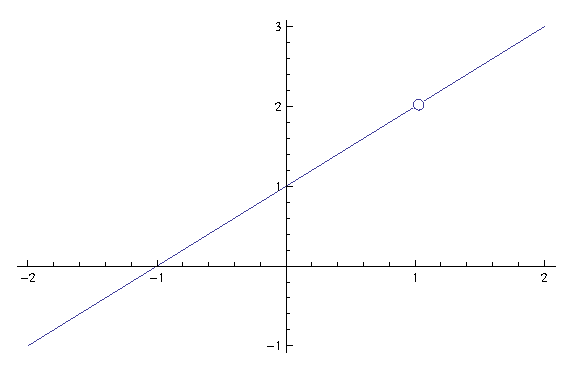
\includegraphics[scale=0.7]{graphs/p1ch3x2m1xm1}
  \end{center}
  \caption{A plot of \(f\). Note the hole at \(x=1\).}
\end{figure}
However, we may still wish to know how the function behaves \emph{around} \(x=1\).
This is where limits come in handy.
They discuss the behavior of a function near a specific point, without any consideration for how the function behaves exactly \emph{at} that point.
To find the behavior of \(f\) around \(x=1\), we take the limit of \(f\) as \(x\) approaches \(1\).
\begin{defn}\label{defn:limi}\index{limit definition}
  \( \lim_{x \to a} f(x) = L \) if and only if \(f(x)\) gets \emph{arbitrarily} close to \( L \) as \(x\) gets \emph{sufficiently} close to \(a\).
\end{defn}
\begin{remark}
  In this case, \textbf{arbitrarily close} implies that we can make the number as close as we could possibly request it. \textbf{sufficiently close} means that we can find a number $x$ where, for every number after (or before) it, we are past our arbitrary value of closeness.
\end{remark}
We would write this as:
\[ \lim_{x \to 1} \frac{x^2-1}{x-1} \]
In this case, we can evaluate this using basic algebra to simplify the original function,
\begin{align*}
   f(x)&=\frac{x^2-1}{x-1} && x \neq 1 \\
   &=\frac{(x+1)(x-1)}{x-1}&& x \neq 1 \\
   &=x+1 && x \neq 1
\end{align*}
\begin{remark}
  We must make the statement that $x \neq 1$ whenever $x+1$ is in the denominator of a function,
  because if $x$ could ever be equal to $1$, it would make the value of $f(x)$ undefined at this point.
\end{remark}
Then we define a new function equivalent to the above, but where \(1 \in D\).
We then evaluate our new function at \(x=1\).
\[ g(x) = x+1 \]
Which gives us
\begin{align*}
  \lim_{x \to 1} \frac{x^2-1}{x-1}
  &=g(1)
  \\&=2
  \text{.}
\end{align*}

It turns out we have a number of rules that describe how we can go about
evaluating a limit.
\begin{theorem}[Limit Laws]
  If \(L\), \(M\), and \(k\) are real numbers and
    \[ \lim_{x \to c} f(x)=L \quad and \lim_{x \to c} g(x) = M \]
  then,
  \begin{table}[H]
    \centering
      \begin{tabular}{p{3in}>\(p{3in}<\)}
        Sum Rule: & \displaystyle{\lim_{x \to c} (f(x) + g(x)) = L + M} \\ \\
        Difference Rule: & \displaystyle{\lim_{x \to c} (f(x) - g(x))=L-M} \\ \\
        Constant Multiple Rule: & \displaystyle{\lim_{x \to c} (k \cdot f(x)) = k
      \cdot L} \\ \\
      Quotient Rule: & \displaystyle{\lim_{x \to c} \frac{f(x)}{g(x)} =
      \frac{L}{M}, \quad m\neq 0} \\ \\
      Power Rule: & \displaystyle{\lim_{x \to c} [f(x)]^n = L^n, \quad n \in
      \mathbf{Z_+}} \\ \\
      Root Rule: & \displaystyle{\lim_{x \to c} \sqrt[n]{f(x)} =
      \sqrt[n]{L}=L^{1/n}, \quad n
    \in Z_+}
  \end{tabular}
  \end{table}
  If \(n\) is even, we assume that \(\lim_{x \to c} f(x) = L > 0\). This is because for the rules including exponents, for $\lim{x\to c} f(x)=L<0$ to be true we would require imaginary numbers.
\end{theorem}

Not all functions have limits defined everywhere on their domain.
For example, \(h(x)=\sin \frac{1}{x} \) oscillates indefinitely as \(x \to 0\), as shown in Figure \ref{fig:p1sin1x}.
\begin{figure}[H]
  \begin{center}
    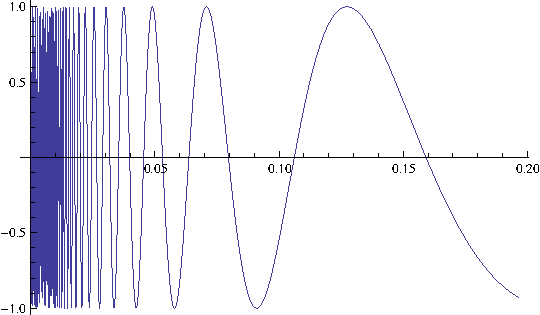
\includegraphics{graphs/p1sin1x.pdf}
  \end{center}
  \caption{The limit of \(h(x)\) as \(x \to 0\) does not exist.}
  \label{fig:p1sin1x}
\end{figure}
As \(x\to0\), it is impossible to say whether \(f(x)\) is approaching \(1\) or \(-1\).
This is an example of an \textbf{oscillating discontinuity}\index{oscillating discontinuity}.
There are more situations in which a limit does not exist.

In a \textbf{infinite discontinuity}\index{infinite discontinuity}, the graph jumps to $\infty$ or $-\infty$ at certain $x-values$.
No limit can exist here.
\begin{figure}[H]
  \begin{center}
    \includegraphics[width=0.4\textwidth]{continuous/limits/infinited}
  \end{center}
  \caption{An infinite discontinuity at $x=0$.}
\end{figure}

The other situation which can cause a limit to not exist at a point is a \textbf{jump discontinuity}\index{jump discontinuity}.
\begin{figure}[H]
  \begin{center}
    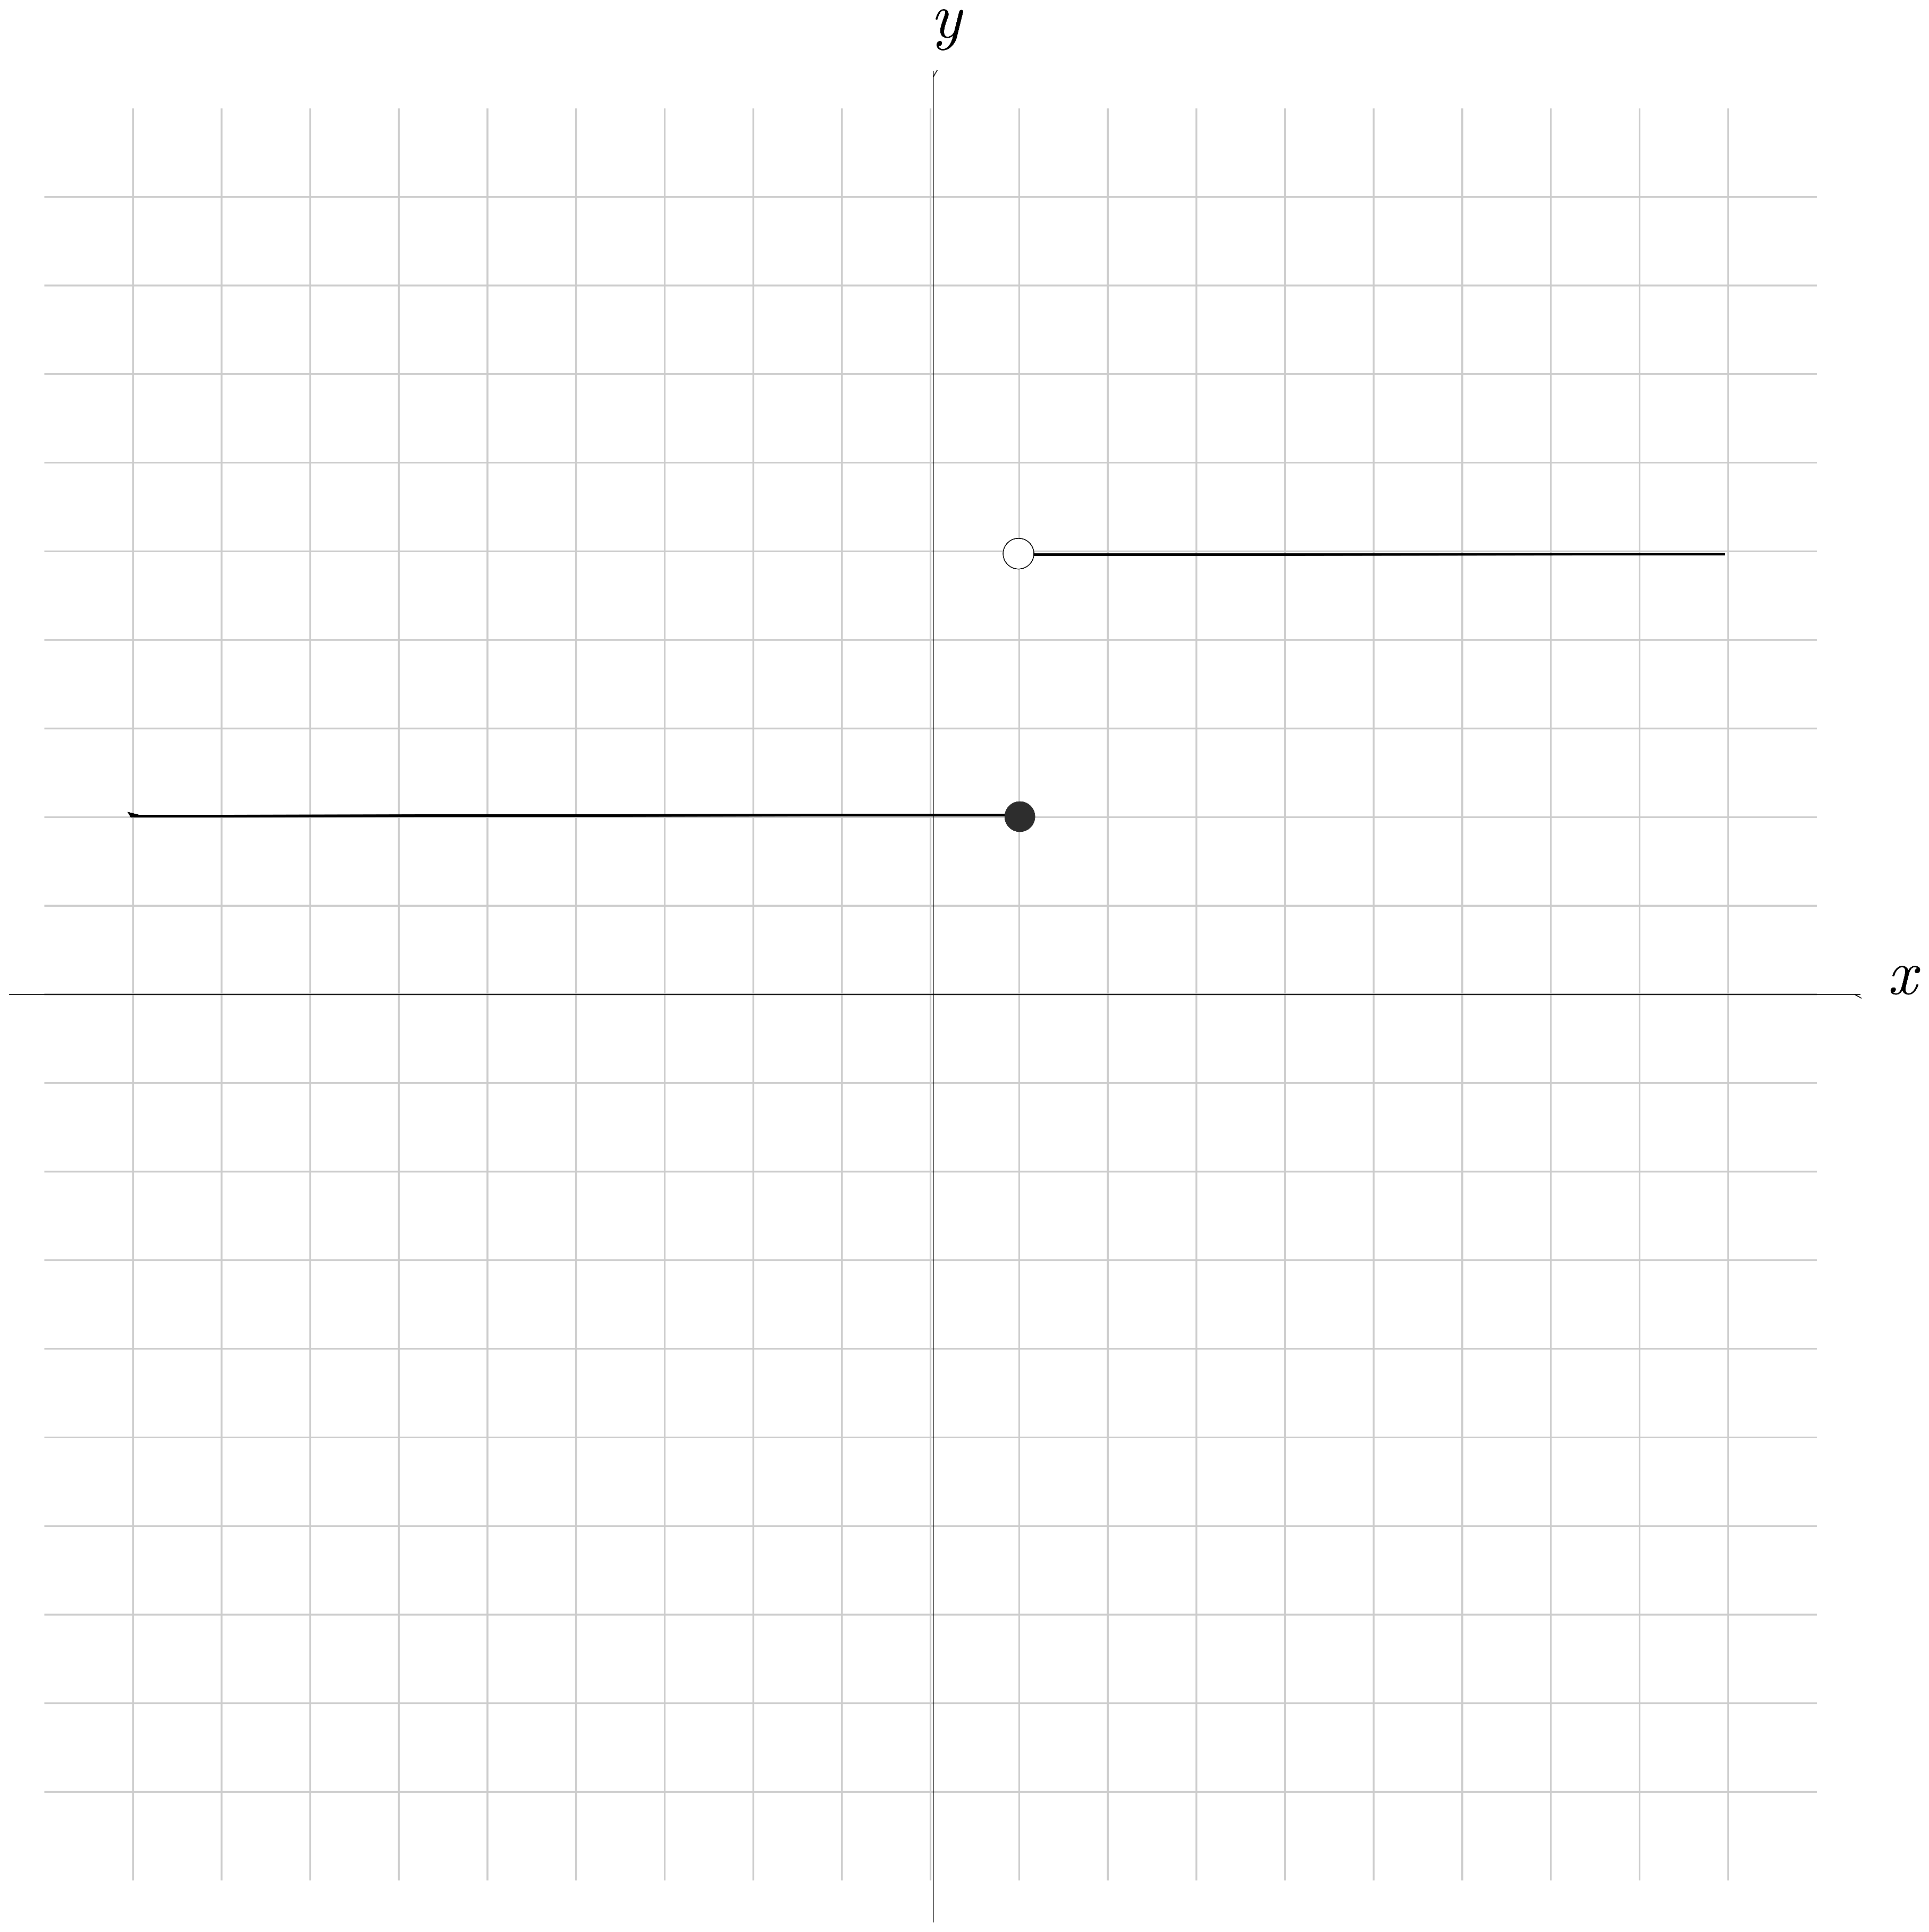
\includegraphics[width=0.3\textwidth]{continuous/limits/jumps}
  \end{center}
  \caption{A jump discontinuity.}
\end{figure}
\subsection{Side Limits}\index{side limits}

In places where a limit does not exist, we can still talk about the limit from just one side or another.
Note, however, that if $\lim_{x\to a}f(x)$ at a point, then the left an right limits also exist and must be equal to one another.

\begin{theorem}
  \( \lim_{x\to a^-} f(x)=L \) iff \(f(x)\) gets arbitrarily close to \(L\) as \(x\) comes sufficiently close to \(a\), but \(x < a \).
  \label{theorem:lefthandlimit}
\end{theorem}
\begin{figure}[H]
  \begin{center}
    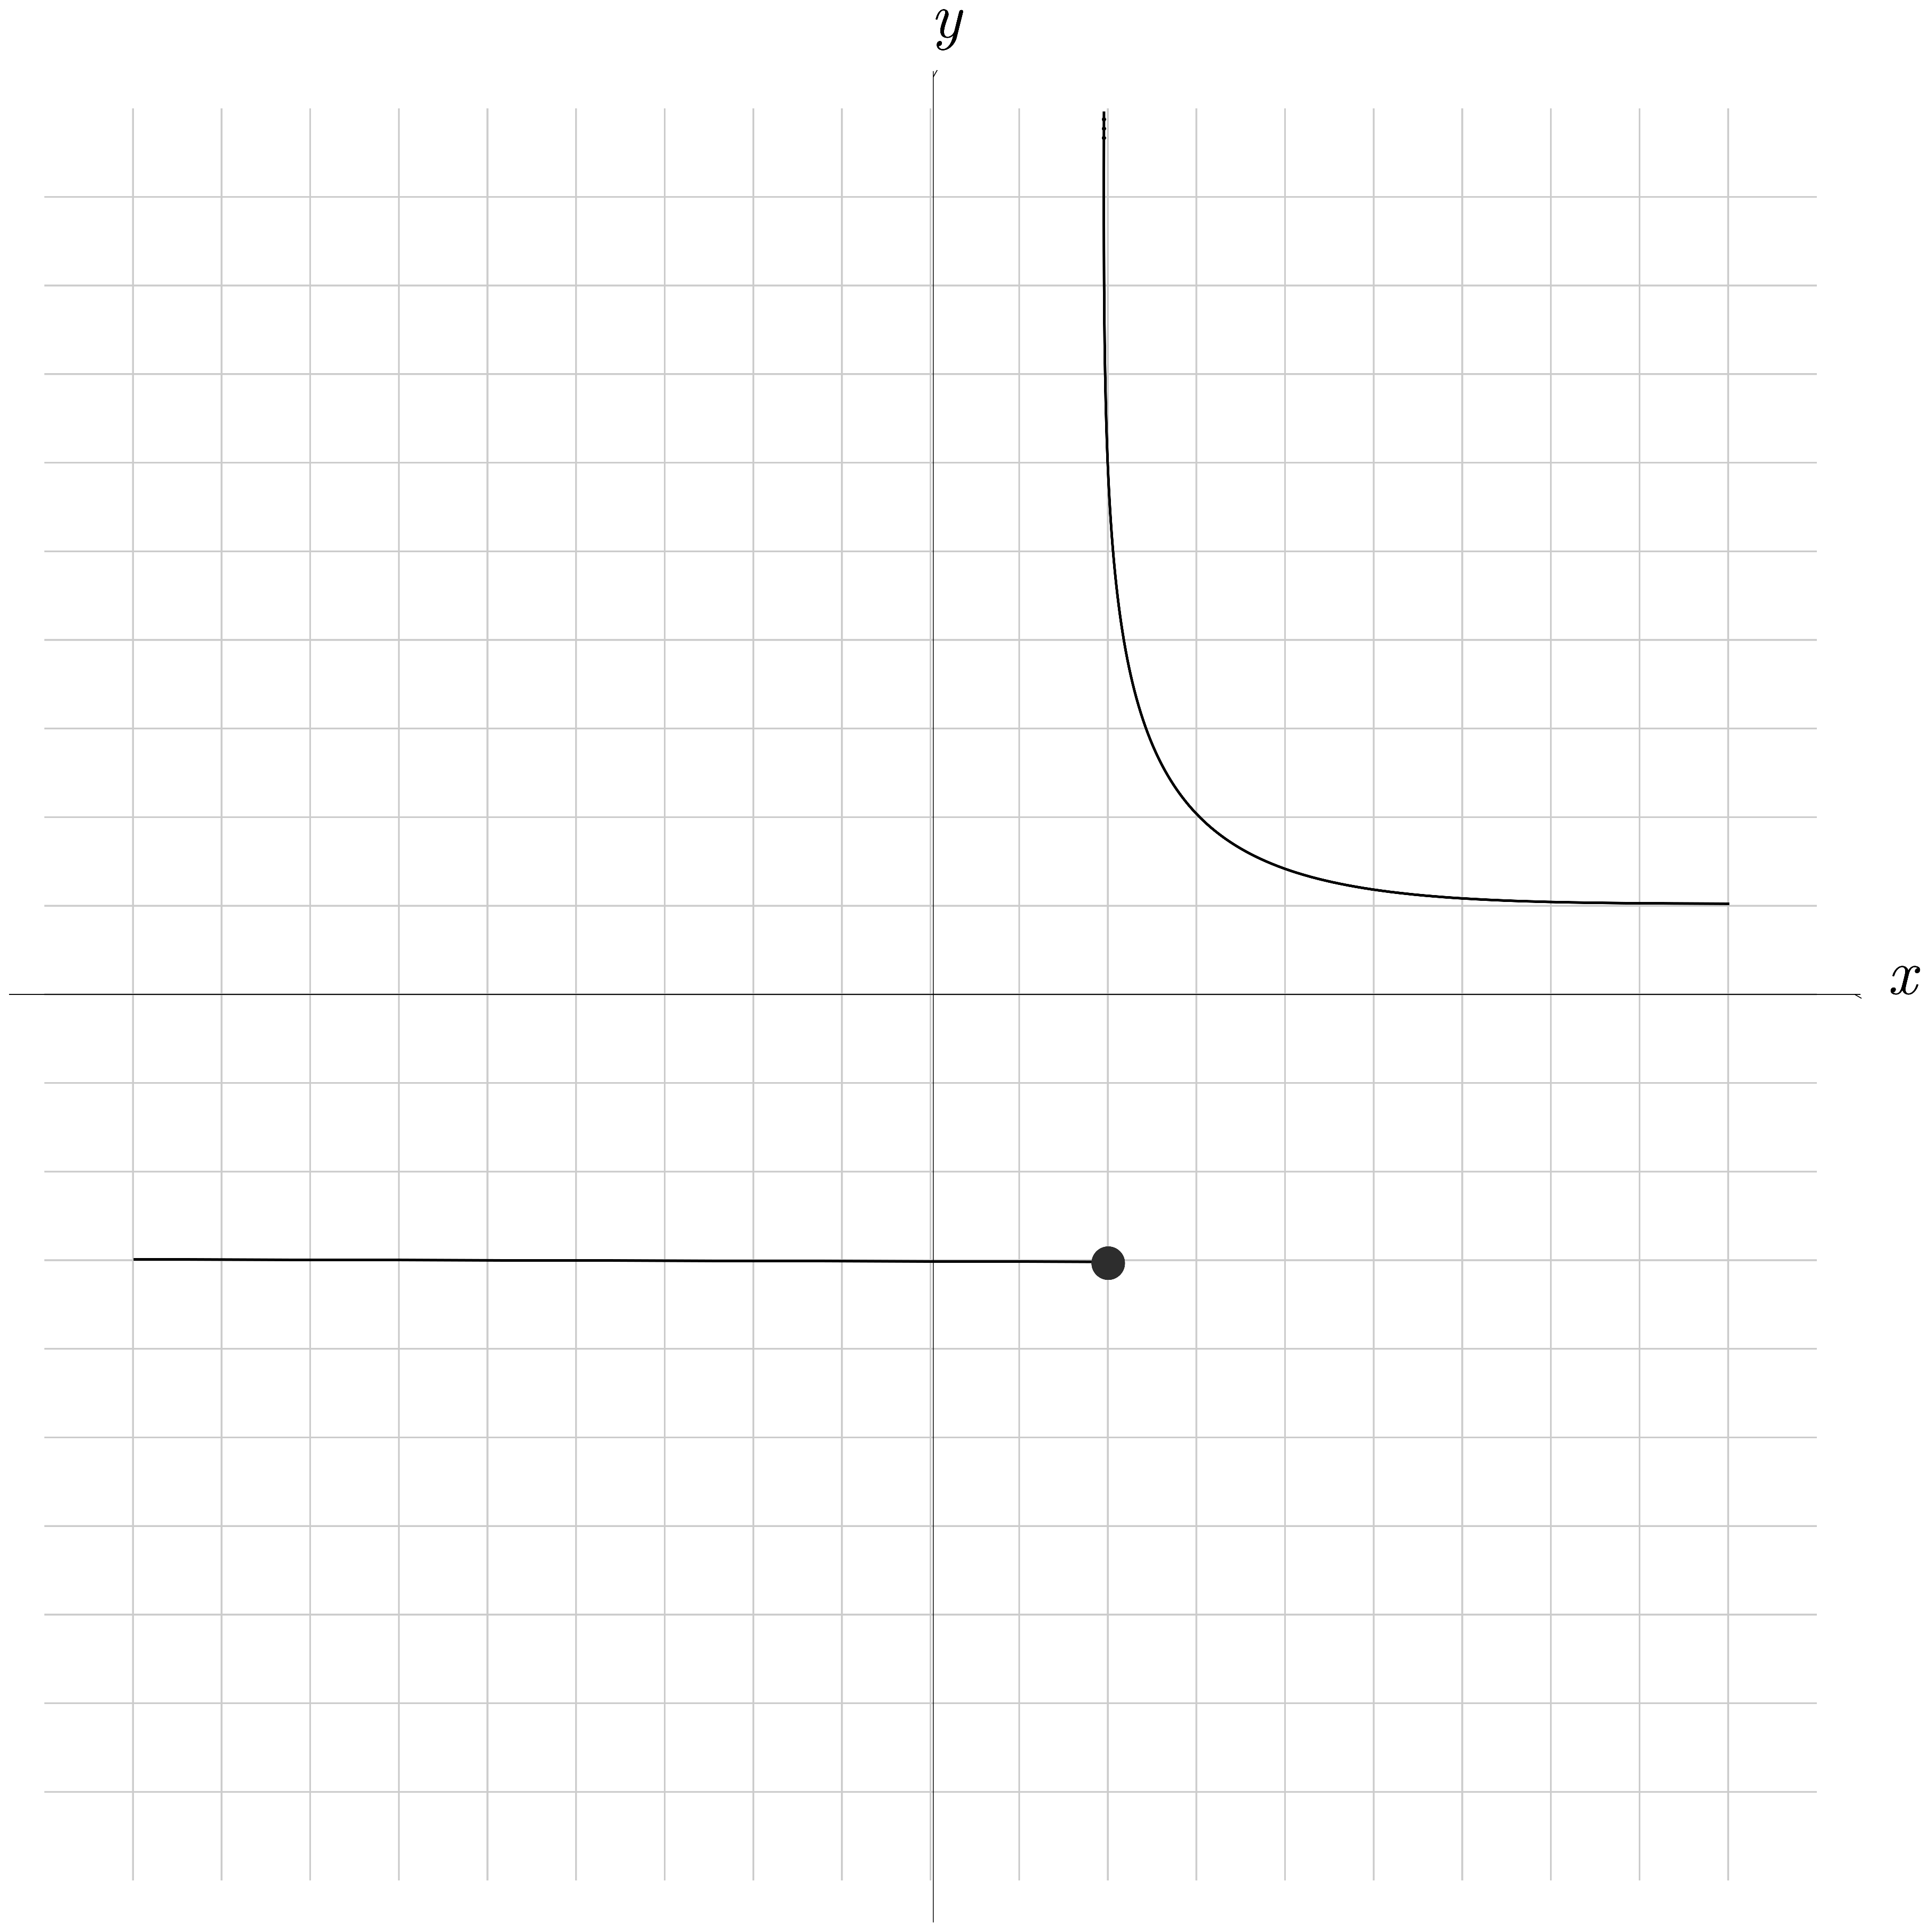
\includegraphics[width=0.5\textwidth]{continuous/limits/llmt}
  \end{center}
  \caption{The lefthand limit at $x=2$ exists, though the righthand limit does not.}
\end{figure}
\begin{theorem}
  \( lim_{x \to a^+} f(x)=L \) iff \(f(x)\) gets arbitrarily close to \(L\) as \(x\) gets sufficiently close to \(a\), but \(x > a\).
  \label{}
\end{theorem}
% section ref: Thomas' Calculus, Chapter 1

\subsection{The Sandwich Theorem}

Let us look at a more complicated example of a limit.
Suppose we have the functions
\begin{align*}
  h(x) &= |x|, \\
  f(x) &= x\sin{\frac{1}{x}}, \\
  \text{and }g(x) &= -|x|,
\end{align*}
where at \(x=0\), \(g(x) \leq f(x) \leq h(x)\) at 0.
\begin{figure}[H]
  \begin{center}
    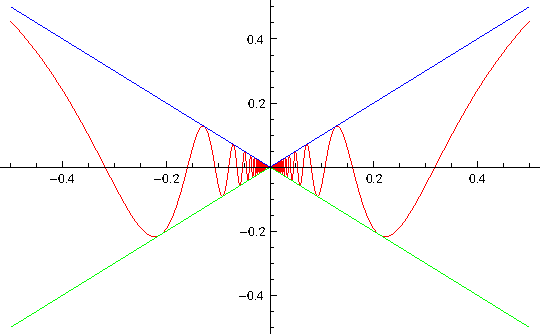
\includegraphics{graphs/sandwichtheorem.pdf}
  \end{center}
  \caption{A plot of \(h(x)\), \(f(x)\), and \(g(x)\)}
\end{figure}
We can conclude, intuitively, that the limit of \(f(x)\) as \(x \to 0\) must be
0 even though we cannot evaluate \(f(x)\) at 0, as seen in Figure
\ref{fig:p1sin1x}. We can generalize this kind of behavior as a theorem, the
\emph{sandwich theorem}.
\begin{theorem}[The Sandwich Theorem]
  If \[g(x) \leq f(x) \leq h(x)\] holds for all \(x \neq c\) in some open interval containing a number \(c\),
  and
  \[ \lim_{x \to c} g(x) = \lim_{x \to c} h(x) = L, \]
  then \(\lim_{x \to c} f(x)\) also equals $L$.
  \label{th:sandwich}
  \index{sandwich theorem}
\end{theorem}

\section{\emph{Epsilon}-\emph{Delta} Definition of a Limit}\index{epsilon-delta definition of a
limit}

The statement
\[ \lim_{x \to a} f(x) = L \]
is the statement
\begin{equation}
  \forall (\varepsilon > 0) \exists (\delta>0) \forall x \Big(0 < | x -a| < \delta \implies
  \big|f(x)-L\big| < \varepsilon\Big),
  \label{eq:e_d_limit}
\end{equation}
where the domain for the variables for $\delta$ and $\varepsilon$ consists of
all positive real numbers and for $x$ consists of all real
numbers.

\section{Evaluating Limits}

Let's look at a really complicated example of a limit\footnote{Credit for this example goes to Dr. Dobrescu's Math 140 class at CNU, Spring 2011.}, to make sure we truly understand them.
For piecewise-defined functions, limits can get especially interesting. Here's an example:
\index{piecewise function}

\begin{ex}
  \[ f(x)=
    \begin{dcases}
      x &: x \in \left[ -1,0 \right) \\
      -x &: x \in \left (0,1 \right) \\
      x-1 &: x \in \left[1, 2\right]
    \end{dcases}
    \]
  \begin{figure}[h]
    \begin{center}
      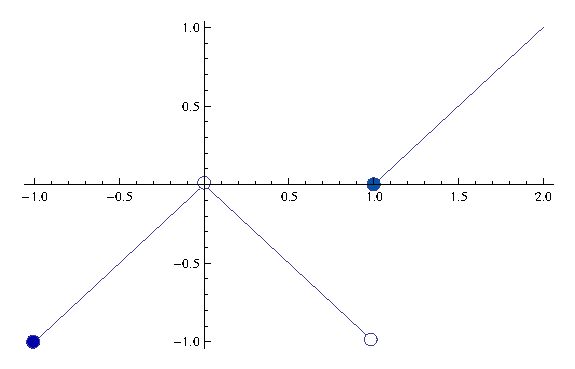
\includegraphics{graphs/pwlimex1}
    \end{center}
    \caption{A graph of \(f(x)\)}
    \label{fig:pwlimex1}
  \end{figure}
  \begin{enumerate}
    \item Does \( \lim_{x\to 0} f(x) \) exist?

      \begin{sol}
        Yes.
      \end{sol}
    \item Does \( \lim_{x \to 0} f(x)=0 \)?

      \begin{sol}
        Yes.
      \end{sol}
    \item Does \(\lim_{x \to 0} f(x)=1\)?

      \begin{sol}
        No. \(\lim_{x \to 0} f(x)=0\).
      \end{sol}
    \item Does \(\lim_{x \to 1} f(x)=1\)?

      \begin{sol}
        No. \( \lim_{x \to 1} f(x) \) does not exist.
      \end{sol}
    \item Does \(\lim_{x \to 1} f(x)=0\)?

      \begin{sol}
        No. The limit does not exist.
      \end{sol}
    \item Can we take \( \lim_{x \to x_0} f(x)\) for every \(\big(x_0 \in (-1, 1)\big)\)?

      \begin{sol}
        Yes.
      \end{sol}
    \item Does \( \lim_{x \to 1} f(x) \) exist?

      \begin{sol}
        Yes.
      \end{sol}
  \end{enumerate}
\end{ex}
\begin{ex}
  Find
  \[ \lim_{x \to 4} \frac{4x-x^2}{2-\sqrt x} \text{.} \]
  \begin{sol}
    \begin{figure}[h]
      \begin{center}
        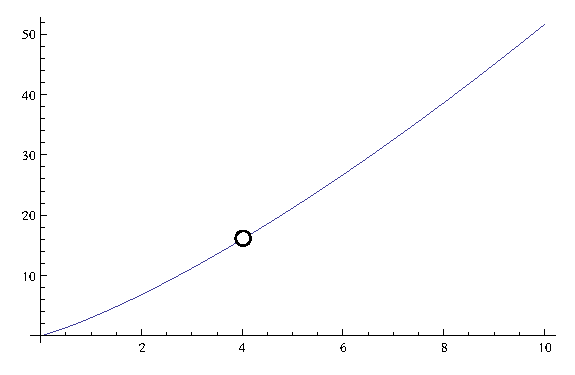
\includegraphics[width=0.4\textwidth]{continuous/limits/4xmx2}
      \end{center}
      \caption{A plot of $f(x)= \frac{4x-x^2}{2-\sqrt x}$.}
    \end{figure}
    First we multiply by the conjugate of the denominator to remove the radical from it. For more detail on conjugates, see Section \ref{app:def:conjugate}.
    \begin{align*}
      \lim_{x \to 4} \frac{4x-x^2}{2-\sqrt x}
      &= \lim_{x \to 4} \frac{4x-x^2}{2-\sqrt x} \cdot \frac{2+\sqrt x}{2+\sqrt x}\\
      \intertext{Then we simplify.}
      &=\lim_{x \to 4} \frac{x\big(4-x\big)\big(2+\sqrt{x}\big)}{4-x}
       = \lim_{x \to 4} \frac{x\big(2+\sqrt{x}\big)}{1} \\
      &= 16
    \end{align*}
  \end{sol}
\end{ex}
\begin{ex}
  Evaluate
  \[ \lim_{x \to -1} \frac{\sqrt{x^2+8}-3}{x+1} \text{.} \]
  \begin{sol}
    \begin{align*}
      \lim_{x \to -1} \frac{\sqrt{x^2+8}-3}{x+1}
      &= \lim_{x \to -1} \frac{\sqrt{x^2+8}-3}{x+1} \cdot \frac{\sqrt{x^2+8}+3}{\sqrt{x^2+8}+3}
      = \lim_{x \to -1} \frac{x^2+8-9}{(x+1)(\sqrt{x^2+8}+3} \\
      &= \lim_{x \to -1} \frac{(x-1)(x+1)}{(x+1)(\sqrt{x^2+8}+3)}
      = \lim_{x \to -1} \frac{x-1}{\sqrt{x^2+8}+3} \\
      &= \frac{-1}{3}
    \end{align*}
  \end{sol}
\end{ex}
\begin{ex}
  Suppose we wished to evaluate the limit
  \[  \lim_{\theta \to 0} \frac{\sin \theta}{5 \theta}. \]
  \begin{sol}
    Well, first we should recognize that $\sin \theta$ is not the kind of function that is growing indefinitely:
    it oscillates forever between two values, $1$ and $-1$.
    \begin{figure}[H]
      \begin{center}
        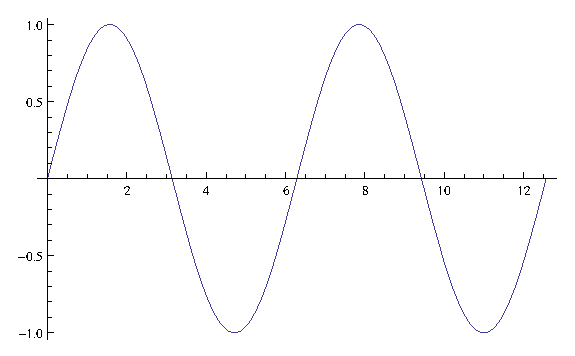
\includegraphics[width=0.5\textwidth]{continuous/limits/sintheta}
      \end{center}
      \caption{A plot of $\sin \theta$.}
      \label{fig:sintheta}
    \end{figure}
  \end{sol}
  But dividing by larger and larger values is going to make this function's \textbf{amplitude}\index{amplitude},
  its distance from the $y$-value of $0$, much smaller.

  Using Theorem \ref{th:sandwich},\footnote{How?} we can see that this limit approaches $1$.
\end{ex}

\section{Indeterminate Forms}

If we want to know how the function
$$F(x)=\frac{x-\sin x}{x^3}$$
behaves \emph{near} $x=0$ (where it is undefined), we can examine the limit of $F(x)$ as $x \to 0$. We cannot apply the Quotient Rule for limits because the limit of the denominator is $0$. Moreover, in this case, \emph{both} the numerator and denominator approach $0$, and $0/0$ is undefined. Such limits may or may not exist in general, but the limit does exist for the function $F(x)$ under discussion by applying l'Hospital's Rule, which is detailed further in Section \ref{sec:lhospital}.

If the continuous functions $f(x)$ and $g(x)$ are both zero at $x=a$, then
$$\lim_{x \to a} \frac{f(x)}{g(x)}$$
cannot be found by substituting $x=a$. The substitution produces $0/0$, a meaningless expression, which we cannot evaluate. We use $0/0$ as a notation for an expression known as an \textbf{indeterminate form}. Other meaningless expressions often occur, such as $\infty / \infty$, $\infty \cdot 0$, $\infty - \infty$, $0^0$, and $1^{\infty}$, which cannot be evaluated in a consistent way; these are called indeterminate forms as well.

\section{Continuity of Functions}
\begin{defn}
  A function is \textbf{continuous}\index{continuous} at $x=a$ iff
  \begin{itemize}
    \item $f(a)$ is defined.
    \item $\lim_{x\to a} f(x)$ exists.
    \item $\lim_{x\to a} f(x)=f(a)$.
  \end{itemize}
\end{defn}

\section{The Mean Value Theorem}
\index{mean value theorem}
The following is a simplified case of the mean value theorem:
The \textbf{mean value theorem} states that, for a continuous function $f$,
if we have an $f(a)$ which is negative and a $f(b)$ which is positive,
then $f$ crosses the $x$-axis somewhere on the interval $(a, \, b)$.
